\documentclass[10.5pt,a4paper]{ctexart}
\usepackage[margin=2.0cm]{geometry}
\usepackage{amsmath,amssymb,booktabs,longtable,tabularx,array,enumitem}
\usepackage{xcolor,hyperref,xurl,tikz,listings}
\usetikzlibrary{arrows.meta,positioning,fit,calc}
\hypersetup{colorlinks=true,linkcolor=blue!55!black,urlcolor=blue!55!black}
\setlength{\emergencystretch}{2em}
\setlist[itemize]{leftmargin=2em,itemsep=0.2em,topsep=0.3em}
\setlist[enumerate]{leftmargin=2.2em,itemsep=0.2em,topsep=0.3em}
\definecolor{smblue}{RGB}{50,100,155}
\definecolor{pmorange}{RGB}{194,105,45}
\definecolor{proofgreen}{RGB}{52,125,83}
\definecolor{soft}{RGB}{244,247,250}
\newcolumntype{L}[1]{>{\raggedright\arraybackslash}p{#1}}
\newcommand{\term}[1]{\textbf{#1}}
\newcommand{\code}[1]{\texttt{#1}}
\newcommand{\caveat}[1]{\par\smallskip\noindent\colorbox{soft}{\parbox{0.95\linewidth}{\textbf{边界：}#1}}\par\smallskip}
\newcommand{\todo}[1]{\par\smallskip\noindent\fcolorbox{orange!70!black}{orange!8}{\parbox{0.94\linewidth}{\textbf{成稿前待补：}#1}}\par\smallskip}
\lstset{basicstyle=\ttfamily\small,breaklines=true,columns=fullflexible,frame=single}

\title{TrainVerify：由 Lean 内核检查的编译器生成分布式训练图等价性\\\large 中文技术报告初稿 v0.2}
\author{TrainVerify 项目}
\date{2026 年 8 月 11 日}

\begin{document}
\maketitle

\begin{abstract}
分布式训练编译器把单设备训练程序改写成多张设备局部程序，并插入张量分片、复制、通信、布局变换与调度。程序能够运行、张量形状一致或少量随机测试通过，都不能说明改写前后计算的是同一个值：两个局部张量可能拥有完全相同的形状，却分别代表连续序列分片、首尾交错的 zigzag 分片、复制副本或不同专家持有的 token。TrainVerify 将这类正确性问题转换为 Lean 可检查的关系命题。系统从固定源码和真实双 GPU 运行中取得单设备参考图 SM 与并行执行图 PM，把图节点、张量值、设备所有权和 collective 翻译成形式语义，沿目标的完整上游依赖生成命题，再把局部算子关系组合为图级证明。

本文从分布式训练的基本对象开始，解释 llm-train 如何定义 YOCO 模型，nnScaler 如何 trace、规划、插入 adapter 和 collective 并生成 SM/PM，以及这条转换为什么容易产生 shape-correct but value-wrong 的错误。随后给出 TrainVerify 的图翻译、人工 fidelity audit、命题构造、proof-certificate composition、信任边界和发布机制。YOCO-MoE-A0.4B 案例在固定 revision 的真实双 GPU authority 上得到五个公开 full theorem；最终快照直接检查 463 个 Lean 模块，并以逐文件 registry 和 receipt 绑定图来源、证明源码与检查结果。该结果证明的是项目张量语义下五个固定 observable 的关系，不是 CUDA kernel 的逐位等价、完整训练收敛或任意网络的一键验证。本文最后把已经通用、设计上应通用但尚未完成、以及必须由模型或框架专家单独投入的工作明确分开。
\end{abstract}

\section{引言}

考虑长度为 8 的序列。普通两路切分可以让 rank 0 持有行 $[0,1,2,3]$，rank 1 持有 $[4,5,6,7]$；按 rank 顺序执行 AllGather 能恢复原序列。context parallelism 使用的 zigzag 布局却可能让两个 rank 分别持有 $[0,1,6,7]$ 与 $[2,3,4,5]$。两种情况下，每个局部张量的 shape 完全相同，但普通 rank-order concat 在后一种布局下得到
\[
[0,1,6,7,2,3,4,5],
\]
而不是原序列。通信调用可以成功，输出 shape 也正确，错误却已经进入值语义。

这不是孤立的排列问题。现代训练框架会组合 tensor parallelism、expert parallelism、context parallelism 和 data parallelism。编译器需要决定每个张量由哪些 rank 持有、沿哪一维切分、何时复制、何时 reduce，以及在两种布局之间插入什么 adapter。MoE 还要处理 token routing、expert ownership 和 AllToAll；ring或sliding-window attention还会让 query stream 与 cache K/V 采用不同布局。任何一层的 annotation、partition、input order、process-group scope 或重构规则出错，都可能得到“能运行但计算了另一个函数”的程序。

传统测试覆盖了其中一部分风险。shape checking 能发现维度不一致；CPU smoke 能发现 import、trace 和 code generation 失败；数值 differential testing 能在有限输入上比较输出。但这些方法无法穷尽所有 rank-local 值关系，也很难判断测试没有触发的布局分支。另一方面，直接对训练框架源码做完整形式化成本过高，而且真实并行计划依赖 compiler revision、cost profile、硬件和 runtime path。TrainVerify 选择一条 translation-validation 路线：固定一次真实编译得到的 SM/PM 图，为该图建立值语义，并由 Lean 检查“PM 的局部值能否按声明的布局关系重构为 SM 值”。

本文作出以下贡献。
\begin{enumerate}
  \item 给出一种面向分布式训练图的值级规格。它不仅记录 shape，还显式区分连续分片、zigzag、复制、expert ownership、hidden sharding 和 collective scope。
  \item 给出 authority-backed graph-to-Lean pipeline。系统将真实 llm-train/nnScaler 编译产物、硬件与 profile provenance、图结构和目标 observable 转换为声明、输入条件和 proof obligations。
  \item 给出从局部算子关系到完整目标上游依赖的证明组织方法。命题从真实外部输入开始，不允许把图计算产生的中间值作为未经约束的 premise。
  \item 在 YOCO-MoE-A0.4B 的真实双 GPU 图上闭合五个公开 full theorem，并建立 theorem-header、axiom、non-vacuity、all-source build、registry 和 sealed receipt 门禁。
  \item 系统分析当前方法的泛化边界，区分可复用语义库、尚未自动化的 relation inference 与 certificate synthesis，以及新算子、新布局和新训练框架不可避免的人工 fidelity audit。
\end{enumerate}

图~\ref{fig:pipeline}给出全文主线。需要特别注意，Lean theorem、GPU authority 和 sealed publication 是三层不同证据。Lean 检查 proof term 是否证明给定声明；authority 说明声明里的图来自哪次真实编译；publication 说明被检查和被发布的是同一组字节。任何一层都不能替代另外两层。

\begin{figure*}[t]
\centering
\resizebox{\textwidth}{!}{%
\begin{tikzpicture}[node distance=6mm and 8mm,>=Latex,
 box/.style={draw,rounded corners,minimum height=9mm,align=center,font=\small,fill=white},
 arr/.style={->,thick}]
\node[box,fill=smblue!10] (src) {llm-train\\模型与训练代码};
\node[box,right=of src,fill=smblue!10] (trace) {nnScaler\\trace 与 IRGraph};
\node[box,right=of trace,fill=pmorange!12] (plan) {PAS/AutoDist\\分区与 adapter};
\node[box,right=of plan,fill=pmorange!12] (graph) {真实双 GPU\\SM/PM authority};
\node[box,right=of graph,fill=proofgreen!12] (lean) {GraphDecl、Denote\\relations 与 goals};
\node[box,right=of lean,fill=proofgreen!12] (proof) {certificate DAG\\Lean kernel};
\draw[arr] (src)--(trace); \draw[arr] (trace)--(plan); \draw[arr] (plan)--(graph);
\draw[arr] (graph)--(lean); \draw[arr] (lean)--(proof);
\node[below=5mm of graph,font=\footnotesize,align=center] {固定 revision、硬件、通信/算子 profile、SM/PM rank-0 capture receipts};
\node[below=5mm of lean,font=\footnotesize,align=center] {不可信生成器；声明与证书由 Lean 检查};
\end{tikzpicture}%
}
\caption{从训练源码到内核检查证明的端到端链。}
\label{fig:pipeline}
\end{figure*}

\section{分布式训练入门}

\subsection{一次训练迭代里有哪些对象}

为了理解 SM 和 PM，不需要先掌握完整的深度学习数学。一次训练迭代至少包含四类对象。

第一类是\term{外部输入}，例如 token、label、packed sequence metadata 和 attention mask。第二类是\term{参数}，例如 embedding matrix、attention projection 和 MoE expert weights。第三类是\term{中间张量}，它们由 forward operators 依次产生。第四类是\term{梯度与更新状态}，由 loss 反向传播得到。编译器 trace 的图不一定只包含模型论文里的“层”；它还可能包含 reshape、stack、autograd、gradient accumulation、通信和为布局转换插入的 adapter。

YOCO-MoE-A0.4B 中与本文最相关的 forward 路径包括 embedding、24 个 decoder layers、attention、MoE router、expert grouped GEMM、residual、RMSNorm 和 cross-entropy head。context parallelism 会改变序列行的设备所有权，expert parallelism会改变 token 与 expert weight 的设备所有权。两者叠加后，某个 attention layer 可以同时消费 zigzag 的 query stream 和普通连续分片的 cache K/V。

\subsection{rank、shard 与 collective}

\term{rank}是一次分布式执行中的工作进程，通常绑定一张 GPU。一个全局 tensor 可以被复制到所有 rank，也可以沿某个维度分片。\term{collective}是多个 rank 共同参与的通信，例如：
\begin{itemize}
  \item AllGather：收集各 rank 的 shard；
  \item AllReduce：聚合并把结果发送给所有 rank；
  \item ReduceScatter：聚合后再分片；
  \item AllToAll：每个 rank 向每个 rank 发送不同分块。
\end{itemize}

collective 的名字本身不决定正确性。AllGather 必须知道 concat 维度和 rank 顺序；AllToAll 必须知道输入如何切块、输出如何排列；process group 还决定哪些 rank 参与。只要其中一个约定与 producer 的实际 ownership 不一致，就可能产生 shape 正确的错误值。

\subsection{常见并行方式}

\begin{table}[h]
\centering
\small
\begin{tabularx}{\linewidth}{p{0.17\linewidth}X X}
\toprule
方式 & 核心想法 & 对正确性规格的影响 \\
\midrule
Data parallelism & 不同 rank 处理不同样本，参数或梯度同步 & 需要 batch partition 与 gradient reduction 关系 \\
Tensor parallelism & 沿 hidden、head 等维度切分算子 & 需要 shard、partial result 和 gather/reduce 关系 \\
Pipeline parallelism & 不同 rank 执行不同层 & 需要 stage boundary 与调度顺序 \\
Context parallelism & 沿 sequence 切分 attention & 需要 sequence ownership 与 permutation 关系 \\
Expert parallelism & 不同 rank 持有不同 experts & 需要 routing、token dispatch 与 AllToAll 关系 \\
\bottomrule
\end{tabularx}
\caption{并行方式改变的不只是 shape，还包括值的设备所有权和重构方式。}
\end{table}

\section{SM 与 PM 图}

\subsection{SM 图包含什么}

本文把单设备参考图称为\term{SM graph}。SM/PM 是 TrainVerify 对两次独立 nnScaler 编译结果的命名，不是 nnScaler 上游定义的原生对象。SM 也不是手写数学规格，而是同一 BackBone 子模块在单设备计划下 trace、规划和 code generation 得到的参考执行图。抽象上，一张图包含：
\begin{itemize}
  \item 按执行顺序排列的节点；
  \item 每个节点的 operator、输入与输出 tensor ID、参数；
  \item tensor shape 和 producer-consumer edge；
  \item rank、replica group 和 process-group metadata；
  \item 外部输入与目标 observable；
  \item 与源码 revision、pickle 和 profile 绑定的 provenance。
\end{itemize}

SM 的作用是提供未经过目标并行计划改写的参考计算。它不要求与 PM 节点一一对应。一个 SM 节点在 PM 中可以展开成多个 rank-local 节点，也可以由局部算子和 collective 的组合实现。

\subsection{PM 图新增什么}

\term{PM graph}是并行规划器生成的多 rank 执行图。与 SM 相比，它新增或改变：
\begin{itemize}
  \item 节点在哪些 rank 上执行；
  \item tensor 是复制、连续分片、zigzag、expert-local 还是 partial reduction；
  \item 参数和 activation 的 placement；
  \item 为布局不匹配插入的 Chunk、AllGather、AllReduce、AllToAll 等 adapter；
  \item process group、replica-buddy 和 rank-local topology；
  \item runtime 需要的通信与算子 profile。
\end{itemize}

图~\ref{fig:smpm}用一个简化 linear 例子展示二者差异。SM 直接计算 $y=xW$；PM 把 $W$ 沿输出维切成两块，每个 rank 计算一个局部 $y_r$，随后根据下一节点的需要保留 shard 或执行 gather。正确性要求不是两个图长得一样，而是局部输出满足一个可重构关系。

\begin{figure}[h]
\centering
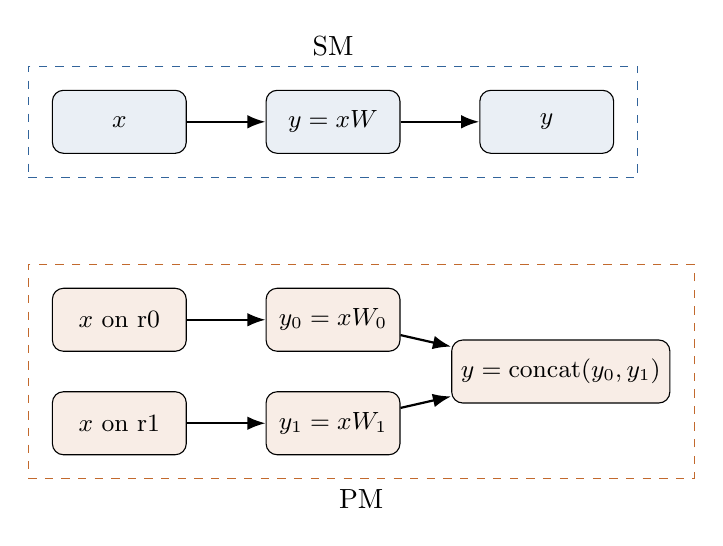
\begin{tikzpicture}[>=Latex,node distance=8mm and 10mm,
 n/.style={draw,rounded corners,minimum width=17mm,minimum height=8mm,align=center,font=\small},a/.style={->,thick}]
\node[n,fill=smblue!10] (x) {$x$};
\node[n,right=of x,fill=smblue!10] (lin) {$y=xW$};
\node[n,right=of lin,fill=smblue!10] (y) {$y$};
\draw[a] (x)--(lin); \draw[a] (lin)--(y);
\node[n,below=17mm of x,fill=pmorange!12] (x0) {$x$ on r0};
\node[n,right=of x0,fill=pmorange!12] (l0) {$y_0=xW_0$};
\node[n,below=5mm of x0,fill=pmorange!12] (x1) {$x$ on r1};
\node[n,right=of x1,fill=pmorange!12] (l1) {$y_1=xW_1$};
\node[n,right=15mm of $(l0)!0.5!(l1)$,fill=pmorange!12] (rel) {$y=\mathrm{concat}(y_0,y_1)$};
\draw[a] (x0)--(l0); \draw[a] (x1)--(l1); \draw[a] (l0)--(rel); \draw[a] (l1)--(rel);
\node[fit=(x)(lin)(y),draw=smblue,dashed,inner sep=3mm,label=above:{SM}] {};
\node[fit=(x0)(x1)(l0)(l1)(rel),draw=pmorange,dashed,inner sep=3mm,label=below:{PM}] {};
\end{tikzpicture}
\caption{SM 与两 rank PM 的简化示例。节点不一一相等，目标是局部值可重构。}
\label{fig:smpm}
\end{figure}

\section{llm-train 与 nnScaler 如何生成 SM/PM}

\subsection{llm-train：被编译的程序}

llm-train 定义 YOCO 模型结构、forward 调用、custom operators、训练输入以及 context/expert parallelism 所需的 API。真实入口不是一个独立的 \code{Trainer.compile()} 方法。\path{nnscaler_train.py --run_mode compile} 构造 \code{TrainerArgs} 后调用 \code{Trainer.run}；\path{Trainer._setup} 在 compile-only 分支以 \path{load_module=False} 调用 \path{parallelize_model}，再进入 \code{ModuleParallelizeConfigAdapter.parallelize}、\code{nnscaler.parallel.parallelize} 和 \path{_gencode}。

被并行化的对象是 \code{BackBone} 子模块，不是完整 \code{WrapperModel}。llm-train 把 \code{BackBone} 注册为唯一 \code{ModuleParallelizeConfig}；nnScaler 在构造 wrapper 时截获该子模块。\code{BackBone.forward} 输出 token loss、routing maps 和 expert probabilities，外层 \code{WrapperModel.forward} 对标量总 loss 的汇总不在捕获的 \code{ModuleCodeGen} 内。最终 SM/PM 因而不包含 optimizer update、dataloader 或完整训练循环。

llm-train还通过 wrapper 或 annotation 告诉 nnScaler 某些 custom op 的输入输出结构。这里必须区分三件事：模型代码规定数学数据流；annotation 描述编译器可以怎样理解和切分 custom op；runtime kernel selector 决定当前硬件实际尝试哪些实现。三者属于不同责任层。

例如，\code{wrap\_maybe\_shuffle(h)} 是否执行真实 permutation，取决于 context-parallel process group 和 world size。K/V projection 在该调用之前还是之后，决定 cache 的 ownership。仅从变量名、所在 layer 或最终 shape 无法可靠推断这一点，必须沿源码和图中的 producer edge 检查。

\subsection{nnScaler：从程序到 IRGraph}

llm-train 的 dummy-sample generator 构造 tokens、targets、positions、packed \path{cu_seqlens}、loss masks、indices 和 length metadata，再由 \path{backbone_forward_args_gen_fn} 包装成 \code{samples} 参数。nnScaler把子模块和这些dummy tensors移至CPU，运行 \path{concrete_trace}，把custom op注册为leaf，随后将FX graph转换成IRGraph。

forward graph来自trace；backward不是一次真实PyTorch训练反传的记录。由于BackBone作为非end-to-end子模块编译，nnScaler随后显式调用 \code{IRGraph.backward(None)}，逆序遍历forward nodes并创建mirror backward ops。捕获的 \code{ModuleCodeGen} 因而包含自动生成的backward节点。

当前Lean release的边界更窄：最终 \path{GeneratedYOCOMoE.lean} 与五个公开Goal只声明并证明forward、adapter和collective组成的目标ancestry，没有把这些backward节点翻译进公开GraphDecl。本文只能声称authority捕获了backward结构，不能声称当前五个theorem验证了backward正确性。

随后，PAS/AutoDist读取用户约束、硬件规模、通信profile和算子computation profile，运行带内存界和通信/计算代价的受约束动态规划搜索，并采用该搜索返回的候选计划。这里不能仅凭 \path{pas_autodist} 名称声称获得数学意义上的全局最优并行方案。

计划为计算节点分配device并执行partition或replicate后，\code{IRAdapterGener} 展开multiref、生成activation adapters与weight reducers。ExecutionPlan按device建立执行序列；DiffFusion与Grouping进一步整理图；\code{ModuleCodeGen}再为每个runtime rank生成 \path{gencode<rank>.py}。nnScaler原生 \path{_gencode} 不生成 \path{mgener.pkl}。TrainVerify使用最小受控补丁，在 \code{ModuleCodeGen} 构造后、逐rank代码生成前，由local rank 0把该对象dill序列化为 \path{sm_mgener.pkl} 或 \path{pm_mgener.pkl}，并把补丁和pickle digest写入receipt。

SM与PM来自同一BackBone源码、输入配置和被认证的profile，但它们不是先生成SM再给它追加通信节点。production generator分别执行两次完整compile：SM使用 \path{plan_ngpus=1, runtime_ngpus=1, zero_group_size=1}；PM使用 \path{plan_ngpus=2, runtime_ngpus=2, zero_group_size=2}。两次都重新经历trace、IRGraph backward、PAS、adapter、ExecutionPlan和ModuleCodeGen。只检查PM无法知道某个collective到底是在实现参考值还是在制造新的值，因此authority和后续验证必须同时保留两侧。

\subsection{profile 为什么也是语义链的一部分}

AutoDist 的选择依赖通信和算子成本。缺失 profile 时使用另一设备的 fallback，或者让正式编译在运行中继续测量并修改 cache，都可能得到另一张 PM 图。TrainVerify 因而把 communication profile、computation profile、GPU inventory 和 planner 配置固定到 authority provenance。profile 不直接证明数学正确性，但它决定被证明的是哪张图。

\subsection{从 nnScaler IR 到 verifier DFG}

TrainVerify 的 Verdict backend 需要把 nnScaler 产物规范化为适合验证的数据流图。这一步不是机械 pickle 序列化。实现需要展开 segment 与 adapter、按 rank 展开节点、规范化 operator、补齐 backward 所需的 forward inputs、处理 constants、强制 single-static-assignment、注入 gradient accumulation，并恢复 shape/value map 与 logical replica identity。

这也是一个高风险翻译边界。历史上实际发现过 reshape target shape 丢失、broadcast shape 用“较长 shape”近似、MoE hidden dimension 从错误参数取得、top-k expert count 解析错误、仅凭 shape 推断 ordinary gather、以及 evaluator selector 只看局部 slice 等问题。它们说明“图能导出”不是翻译正确性的证据。

\section{为什么转换容易出错}

\subsection{shape 不携带 ownership}

图~\ref{fig:layout}展示同一个全局序列的两种两路布局。普通 layout 的重构函数是 rank-order concat；zigzag layout 的重构函数需要把首尾 chunks 重新交错。两种局部 tensor shape 相同，但 relation 不同。

\begin{figure}[h]
\centering
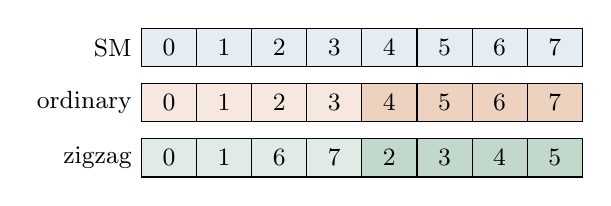
\begin{tikzpicture}[x=7mm,y=7mm,font=\small]
\foreach \i in {0,...,7} {\draw[fill=smblue!12] (\i,2) rectangle +(1,0.7); \node at (\i+0.5,2.35) {\i};}
\node[left] at (0,2.35) {SM};
\foreach \i/\v in {0/0,1/1,2/2,3/3} {\draw[fill=pmorange!15] (\i,1) rectangle +(1,0.7); \node at (\i+0.5,1.35) {\v};}
\foreach \i/\v in {4/4,5/5,6/6,7/7} {\draw[fill=pmorange!30] (\i,1) rectangle +(1,0.7); \node at (\i+0.5,1.35) {\v};}
\node[left] at (0,1.35) {ordinary};
\foreach \i/\v in {0/0,1/1,2/6,3/7} {\draw[fill=proofgreen!15] (\i,0) rectangle +(1,0.7); \node at (\i+0.5,0.35) {\v};}
\foreach \i/\v in {4/2,5/3,6/4,7/5} {\draw[fill=proofgreen!30] (\i,0) rectangle +(1,0.7); \node at (\i+0.5,0.35) {\v};}
\node[left] at (0,0.35) {zigzag};
\end{tikzpicture}
\caption{相同局部 shape 可以对应不同所有权。颜色表示两个 rank。}
\label{fig:layout}
\end{figure}

\subsection{mixed-layout attention}

YOCO 后半段 decoder 是本项目最容易被错误概括的路径。shuffle 后的 Q 与 decoder residual stream 使用 zigzag relation；K/V projection 却在 shuffle 之前完成，因此 cache K/V 仍是 ordinary contiguous shards。attention theorem 必须同时消费 zigzag Q、ordinary K、ordinary V、packed sequence metadata 和真实 reshape semantics。把“同一 layer 里的 tensor”统一标成 zigzag，或者把两个 rank 的 K/V 当复制值，都与实际 producer 顺序冲突。

\subsection{MoE ownership}

MoE router 根据 token 计算 top-k expert indices 与 scores；token 随后被发送到持有对应 expert weights 的 rank。正确性关系需要覆盖 routing map、dispatch mask、remote expert input、grouped GEMM、activation、AllToAll 和 output merge。相似的 operator 名或 TID 不足以证明两个 rank 值相等，replica fact 必须来自共同 source、明确 collective、replica-buddy metadata 或可检查 graph certificate。

\subsection{跨层责任边界}

一次失败可能来自：llm-train 的模型调用或 annotation，nnScaler 的 IR 或 adapter，runtime selector，Verdict normalization，Lean operator denotation，relation choice，statement generation，或者 proof composition。TrainVerify 的失败结果必须保留这些层次，而不是把所有问题统称为“模型 bug”或“证明失败”。

\section{问题定义}

\subsection{图与执行语义}

抽象上，tensor store 是从 tensor ID 到 tensor 值的映射：
\[
\mathrm{Store}=\mathrm{TensorId}\to\mathrm{Tensor}.
\]
图 $G=[n_1,\ldots,n_k]$ 按节点顺序解释。每个节点读取输入 tensor，调用该 operator 的 denotation，再把输出写回 store：
\[
S_{i+1}=\mathrm{evalNode}(n_i,S_i).
\]
目标 $t$ 的图语义记作
\[
\mathrm{denoteGraph}(G,S_0,t)=S_k(t).
\]
对于依赖另一 rank 值、replica group、buddy rank 或 permutation 的节点，普通 rank-local evaluator 不足。faithful distributed evaluator在执行时显式读取跨 rank 结构。

\subsection{关系式正确性}

TrainVerify 不要求 $G_{SM}=G_{PM}$。对目标 observable $o$，证明形式是：若初始 SM store 与各 PM rank store 满足输入条件 $C$，则执行两侧完整上游依赖后，结果满足 relation $R_o$：
\[
\forall S_{SM},S_{PM}^{0},S_{PM}^{1},\quad
C(S_{SM},S_{PM}^{0},S_{PM}^{1})
\Rightarrow
R_o\bigl(\operatorname{eval}(G_{SM},o),
          \operatorname{eval}(G_{PM},o,0),
          \operatorname{eval}(G_{PM},o,1)\bigr).
\]
$R_o$ 可以表示 concat、zigzag reconstruction、复制相等、hidden-shard reconstruction 或更复杂的 collective 结果。

\subsection{威胁模型与非目标}

系统试图发现或拒绝：operator denotation 缺失、relation rule 缺失、ownership 歧义、错误 collective、computed premise 泄漏、statement drift、certificate bug、unexpected axiom、stale artifact 和 provenance mismatch。

系统当前不证明：
\begin{itemize}
  \item CUDA kernel 的逐位浮点等价；
  \item compiler lowering 到 PTX/SASS 的 refinement；
  \item 完整训练收敛、最终模型质量或所有 optimizer state 一致；
  \item 任意 dynamic control flow 或任意 world size；
  \item translator 本身已被形式化验证。
\end{itemize}

\section{TrainVerify 总体设计}

\subsection{Authority capture}

production authority 必须来自真实双 GPU、双 rank NCCL compile path。仅设置 \code{plan\_ngpus=2}、运行 CPU/Gloo smoke、手写 PM graph 或使用单 GPU 都不能替代。真实路径会触发 process group、shuffle、NCCL、GPU profile 和硬件 selector；这些分支可能决定图的 topology。

authority 固定 llm-train、nnScaler 和 TrainVerify revision，记录 GPU、driver、CUDA、NCCL、通信 profile、算子 profile、SM/PM各自的rank-0 capture receipt、pickle hash与节点数。原始 pickle 是可执行输入，emitter 只接受本地产生、权限受控并由 out-of-band hardware digest确认的工件。

\subsection{不可信的声明与证书生成}

Python emitter生成 GraphDecl、shape environment、init goals、input value classes、intermediate obligations、observable goals、manifest 和 path-to-digest ledger。生成器不在 proof core 里；它可以产生任意声明，但不能让 Lean 接受一个类型不正确的 proof term。另一方面，Lean 也不会自动判断声明是否忠实翻译了 authority，因此 graph/semantic fidelity 需要独立审计和 mutation tests。

\subsection{语义库与关系库}

项目为 embedding、linear、RMSNorm、activation、reshape/view、stack、loss、top-k、MoE grouped GEMM、shuffle/unshuffle、attention 和 collective 等建立 denotation，并证明局部 relation-preservation theorems。规则的一般形式是：
\[
R_1(x,x_0,x_1)\land\cdots\land R_m(z,z_0,z_1)\land P
\Rightarrow
R_{out}(f(x,\ldots,z), f_0(\ldots), f_1(\ldots)),
\]
其中 $P$ 是 shape、axis、process group 或 metadata side conditions。

\subsection{命题与证书}

设计目标是：目标生成器从observable同时向后遍历SM和PM producer edges，直到只剩真实外部输入；全图relation inference为每条相关tensor edge选择typed relation；rule selection生成局部obligation；certificate composer再按producer order组成proof DAG。当前YOCO实现只完成了其中一部分：graph declaration、目标slice、backward closure、provenance和若干有限graph certificates可以自动生成；relation选择与长链composition仍混合使用通用theorem、模板化生成模块和YOCO-specific手写proof modules。项目尚未实现对任意受支持图的全图relation inference与完整certificate synthesis。失败时返回结构化诊断仍是设计目标，不是当前所有路径已有的能力。

\begin{figure}[h]
\centering
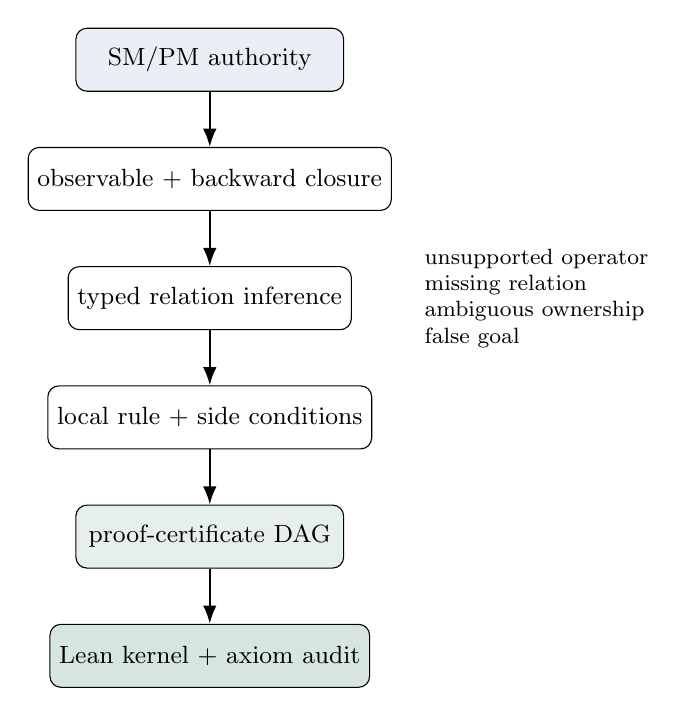
\begin{tikzpicture}[>=Latex,node distance=7mm,
 b/.style={draw,rounded corners,minimum width=34mm,minimum height=8mm,align=center,font=\small},a/.style={->,thick}]
\node[b,fill=smblue!10] (auth) {SM/PM authority};
\node[b,below=of auth] (slice) {observable + backward closure};
\node[b,below=of slice] (rel) {typed relation inference};
\node[b,below=of rel] (rule) {local rule + side conditions};
\node[b,below=of rule,fill=proofgreen!12] (dag) {proof-certificate DAG};
\node[b,below=of dag,fill=proofgreen!20] (kernel) {Lean kernel + axiom audit};
\draw[a] (auth)--(slice);\draw[a] (slice)--(rel);\draw[a] (rel)--(rule);\draw[a] (rule)--(dag);\draw[a] (dag)--(kernel);
\node[right=8mm of rel,align=left,font=\footnotesize] {unsupported operator\\missing relation\\ambiguous ownership\\false goal};
\end{tikzpicture}
\caption{从 authority graph 到 kernel-checked certificate 的逻辑阶段。}
\label{fig:proofpipe}
\end{figure}

\section{翻译忠实性与人工审查}

\subsection{为什么必须有人检查翻译}

Lean 证明的是形式化声明。如果 Python operator 实现为 $f$，Lean 却把它翻译成另一个函数 $g$，那么 $g$ 上的完美证明不能说明 $f$。因此每个新 operator、layout 和 graph adapter 都需要 paper-to-source map。至少要检查：上游源码位置、input/output contract、shape 分支、值公式、world size、process-group scope、Lean declaration、最小可执行例子和 mutation sensitivity。

\begin{longtable}{L{0.17\linewidth}L{0.22\linewidth}L{0.25\linewidth}L{0.25\linewidth}}
\toprule
上游对象 & Lean 对象 & 自动检查 & 人工检查 \\
\midrule
模型/custom op & operator denotation & signature、shape、fixture & 值语义与 Python 源码一致 \\
rank-local tensor & relation instance & producer、rank、shape & ownership、排列和复制来源 \\
collective & transition theorem & group、axis、world size & 与 runtime semantics 一致 \\
目标 slice & goal graph & backward closure & 没有漏 graph-computed input \\
输入条件 & theorem premise & type 与 witness & 条件没有偷渡结论 \\
proof source & registry entry & exact path 与 digest & public theorem owner正确 \\
\bottomrule
\end{longtable}

\subsection{小张量对照与 mutation}

可执行小张量对照能检测常见翻译错误。例如用行号 tensor 检查 shuffle/gather permutation，用非对称 shape 检查 broadcast 和 reshape，用不同 rank 值检查错误 replica assumption。mutation suite 应改变 operator、参数、input order、collective axis、ownership relation 和 certificate，确认系统在预期阶段拒绝。它们提高 fidelity 信心，但仍不等于 translator 已被形式化证明。

\subsection{历史上暴露的 verifier-side 错误}

YOCO 工作实际暴露了多项 verifier-side 问题：MoE grouped GEMM 的 hidden dimension 取错；broadcast 输出 shape 近似错误；top-k experts 参数解析错误；reshape target shape 丢失；仅凭 shape 推普通 gather；evaluator selector没有看到完整 ancestry。每项错误都说明验证器自身也需要测试、审查和fail-closed release，不能把“形式化工具”当作天然正确的裁判。

当前已经对五个headline paths中的关键custom operators、shuffle/unshuffle、ordinary/zigzag relations、MoE ownership和input contracts做过source-level audit，并以这些发现建立回归；但项目尚未发布按全部operator/layout统计的完整fidelity-audit分母、抽样协议和双人审查记录。因此本文不能声称translator已被全面审计。完整coverage与remaining trust assumptions列为RQ1和成稿前门禁。

\section{命题如何生成}

\subsection{完整 backward ancestry}

给定目标 tensor，生成器沿 producer edge 向后闭合。若目标依赖另一 rank 的 collective input，则两侧都必须继续回溯。遍历终点只能是 authority 中的真实 external inputs。旧 cut proof 曾把某个中间 cache 或后 12 层入口 tensor当作 initStore 输入，却没有约束其 lineage；改变该中间值而保持 shape 不变就可能改变最终输出，因此命题过弱。

\subsection{输入条件与 non-vacuity}

合法 caller contract 可以要求 canonical shape、initial shard relation、packed \code{cu\_seqlens} well-formedness、label bounds 等执行前事实。它不能要求“L23 stream 已经满足 Zigzag2Rel”或“某个 loss gather 已相等”，因为这些正是图执行应证明的结果。\code{FivePublicContractsJointWitness} 分别为每个Goal给出一对具体Stores并满足该Goal的全部premises，避免用不可能premise证明任意结论。它不声称同一对Stores同时满足五套shape environment，也不验证真实训练batch必然满足这些conditions。

\subsection{full、cut 与 false findings}

\code{full} theorem 从真实 external inputs 覆盖目标完整依赖；\code{cut} theorem 从中间边界证明局部后缀；legacy/plain theorem可能使用较弱 evaluator。它们可以作为中间结果，但公开名称必须指向 full theorem。

五个公开full theorem不意味着原始obligation全部为真。历史corpus把1151个intermediate TIDs与5个top-level goals组成1156项，其中两条旧Goal 3/4 ordinary rank-order gather等式被zigzag ownership证伪，历史口径为1154/1156。正确处理是保留false finding、在忠实relation下构造新的ancestry-closed命题，并清楚区分“旧命题为假”和“新命题已证”。由于当前coverage脚本与历史corpus已经漂移，1154/1156只作为历史finding分母，不能作为当前release指标；当前release只以五个具名public theorem、registry、axiom audit与final receipt计量。

\section{命题如何证明}

\subsection{局部关系定理}

proof library 把 operator semantics 与输入 relation组合。elementwise operator 通常保持同一 layout；linear 的输出 relation取决于 weight 和 activation 如何分片；reshape必须保持 element order 并更新 shape；shuffle 改变 relation；collective 需要跨 rank 输入；MoE 规则还要使用 routing 与 expert ownership。

\subsection{图级组合}

composer 按 producer order 维护 relation environment。每个 certificate node记录 authority graph fact、选中的 local theorem、premises、side conditions 和 output relation。prefix bridge只有在两图 prefix 可证明相等时使用；filtered bridge只允许忽略目标 backward scope 外节点；Graph A 的事实不能因为 shape 或节点名相似就无桥搬到 Graph B。

\subsection{YOCO 五个公开目标}

Goals 1 和 2 从 embedding 穿过 24 层 decoder、mixed attention、unshuffle、RMSNorm 和 cross-entropy head，复用长 producer prefix但分别证明不同 loss tail。Goal 3 观察 24 层 routing-map stack；Goal 4 观察 24 层 expert-probability stack；两者只在自己的 observable scope 内建立 graph bridge。Goal 5 使用一张较小的完整 ancestry 图，证明 hidden-sharded embedding 与双 rank AllToAll 输出关系。

Goals 1--4 使用 \code{denoteGraphDistributedFaithful}，因为目标 ancestry含跨 rank collective、replica-buddy 或 permutation；Goal 5 使用普通 \code{denoteGraph}，但仍覆盖完整小图。公开入口位于 \code{Instances.lean}，并由 \code{MainTheorem.lean} 聚合。

\subsection{防止“证明错命题”}

release gate逐项检查：
\begin{itemize}
  \item public theorem type 字面等于 \code{goal\_N\_stmt\_full}；
  \item 无 \code{sorry}、\code{sorryAx}、新增手写 axiom 或 \code{False.elim}；
  \item caller contracts有可满足性见证；
  \item final snapshot每个 Lean source都作为 direct elaboration root；
  \item proof registry 固定 exact paths 与 source digests；
  \item stale \code{.olean}、orphan module 和 statement drift 都被拒绝。
\end{itemize}

\section{YOCO-MoE-A0.4B 案例}

\subsection{authority 与图规模}

最终authority来自双NVIDIA RTX PRO 6000 Blackwell、双rank NCCL production run。sealed release对应TrainVerify revision \path{63cabbff6888e3d51359dd2bf9f6d6ae75c2e98a}；此后的文档commit不改变该authority或proof source。固定llm-train revision为
\path{9a1be1d5fd1c063d80be82797692cdc7d23cfbef}，nnScaler revision 为
\path{d3d468ed23edb2f28aa8566b2dfb6ed49c5955cf}。原始 SM 有 2074 nodes，PM 有 4363 nodes。SM/PM raw pickle SHA-256分别为
\path{333a14387e13cb265e74588f02133a0c47b02329d3d1811e6d7a736387494f64}
和
\path{a47d033c83a0cd6dff9111ba49071f3a80eb60869435fc2adeb4f725a71c3462}。

\subsection{证明与发布结果}

最终公开五个full theorem；all-source direct Lean gate检查463个模块；proof registry包含455个模块；exact ledger有456项；emitter tests为54/54，完整Python suite为111/111。registry本身不内嵌在sealed snapshot中，而由final receipt以外部路径和digest绑定。最终manifest digest为
\path{e54a53a32a316ea98e8ee60376ae477f51eebb823355bdb3632de414f1da832d}。

这些数字只描述同一 final receipt绑定的工件。历史 coverage、旧 manifest和早期 candidate snapshot不应与最终结果拼接。

\subsection{发现、撤回与责任边界}

验证过程确认了一项 llm-train CC12 grouped-GEMM selector兼容性问题，也确认了一个历史 nnScaler RVD/annotation/adapter 无法表达 zigzag ownership 的 finding。后者只有双进程 CPU/Gloo 真实源码复现，不能写成 CUDA/NCCL 复现。

调查也产生过两次需要公开的撤回。其一是把 cache K/V 错误推断为 zigzag-owned；源码回溯证明 K/V projection发生在 shuffle 之前。其二是把 trace scope外的 balance-loss consumer用于推断 scope内 goal为假。两项都不能包装成 llm-train语义bug。撤回不是“删掉失败历史”，而是验证方法避免把自己的错误假设固化成正式结论的证据。

\section{实现与信任边界}

\subsection{实现组件}

实现包括 authority generator、nnScaler/Verdict backend、graph-to-Lean emitter、tensor denotation library、relation/proof modules、axiom audit、direct all-source builder、proof registry 和 content-addressed publisher。大型 Lean declaration按语义边界拆分，并限制 direct build worker数量，避免聚合target在高核机器上触发失控并发。

\subsection{可信计算基线}

Lean theorem依赖常规内核项 \path{propext}、\path{Classical.choice} 和 \path{Quot.sound}。有限命题使用 \path{native_decide} 时，还信任 \path{Lean.ofReduceBool} 与 \path{Lean.trustCompiler}。

Python generator、coverage scripts与外部 checker不属于 proof core；它们的输出必须被Lean检查。sealed provenance保证检查和发布的字节一致，但不自动证明从 Python 到 Lean 的语义翻译忠实。

\begin{table}[h]
\centering\small
\begin{tabularx}{\linewidth}{p{0.21\linewidth}X X}
\toprule
层 & 能说明什么 & 不能说明什么 \\
\midrule
GPU authority & 图来自固定revision与真实环境 & 图变换数学上正确 \\
Python emitter & 可复现地产生声明和certificate & 声明忠实且证明成立 \\
Lean kernel/compiler baseline & proof term证明给定声明 & 声明对应真实GPU语义 \\
registry/receipt & 检查与发布字节一致 & operator translation正确 \\
\bottomrule
\end{tabularx}
\end{table}

\section{评估计划与当前证据}

当前YOCO authority捕获了真实、复杂、包含Transformer、MoE、context parallelism、自动生成backward与通信结构的BackBone编译结果；当前Lean声明与五个完整observable只覆盖其中的forward/adapter/collective ancestry，不验证backward节点。它也不覆盖整个WrapperModel、optimizer update、数据加载器或完整训练循环。但一篇OSDI/SOSP论文不能只报告“Lean build通过”。最终评估应围绕以下问题组织。

\paragraph{RQ1：翻译是否忠实？}
对代表性operator、collective与layout运行源码审计、小张量对照和mutation tests，报告每类mutation在哪一层被拒绝。当前已有若干真实verifier-side bug作为回归案例，但仍需系统抽样。

\paragraph{RQ2：覆盖多大规模和哪些语义？}
按faithful denotation、value-lossy legacy与unsupported分类authority节点和obligations；报告nodes、edges、operator classes、relations、proof bytes、Lean时间和peak RSS。五个public theorem与两个false ordinary-gather findings必须同时出现。

\paragraph{RQ3：相比传统检查多发现什么？}
与shape checking、CPU smoke、有限numerical differential test和compiler self-check比较，分析每种方法可见的failure modes。不能把未完成的训练质量影响写进结果。

\paragraph{RQ4：多少工作已经自动化？}
分别统计generated certificates、generic theorem reuse、template-generated modules、model-specific handwritten proof和人工fidelity audit。单一coverage百分比不能代表自动化程度。

\paragraph{RQ5：失败诊断是否有用？}
注入unsupported operator、missing relation、ambiguous ownership、false goal、certificate corruption与provenance mismatch，检查系统是否报告第一个失败node/tensor、expected/actual relation与候选rules。

\paragraph{RQ6：新模型成本是多少？}
至少选择一个未用于开发规则库的architecture做clean-room test，只提供SM/PM authority和contracts。系统应一键生成完整proof，或返回正确分类且可定位的失败。没有该实验前，本文只声称大规模case study和可复用foundation。

\paragraph{RQ7：信任链能否拒绝篡改？}
测试stale \code{.olean}、statement drift、registry corruption、unexpected axiom、impossible contract和pickle/provenance mismatch。

\paragraph{RQ8：开销是否可接受？}
分authority capture、goal generation、certificate generation、Lean elaboration与publication报告cold/incremental时间、CPU、GPU、peak RSS与工件大小。

\todo{当前缺少unseen-architecture clean-room实验、系统化operator fidelity抽样、完整阶段耗时/内存表和公平基线。上述结果未完成前，摘要与结论不得使用“通用proof compiler”。}

\section{泛用性与剩余人工劳动}

\begin{longtable}{L{0.17\linewidth}L{0.23\linewidth}L{0.25\linewidth}L{0.24\linewidth}}
\toprule
变化 & 已可复用 & 应通用但尚未完成 & 必须单独投入 \\
\midrule
新模型，同op/layout & GraphDecl、store、已有语义/关系 & 全图relation inference与certificate synthesis & 目标observable与真实输入contract \\
新operator & 图框架与组合定理 & registry和side-condition plumbing & 源码语义审计与局部定理 \\
新layout & authority和graph traversal & typed relation inference与adapter rules & 重构语义及runtime对照 \\
新训练框架 & Lean core与部分关系库 & 通用IR adapter接口 & graph/provenance extractor \\
新world size & relation抽象的一部分 & 从cp=2推广到参数化rank set & collective scope和permutation证明 \\
新硬件/backend & 抽象operator语义 & 通用authority capture & selector、profile和kernel fidelity \\
\bottomrule
\end{longtable}

已经通用的基础包括GraphDecl、Store、graph fold、部分tensor semantics、若干relations、authority/registry和kernel audit。设计上应当通用但当前仍特化的核心包括typed rule registry、graph-wide ownership inference、proof-certificate DAG synthesis、failure localization、counterexample extraction和参数化world size。当前实现还带有\code{num\_dp=1}、\code{num\_mb=1}等范围限制，bridge emitter也只支持已经实现的topology families。

不可避免的人工工作包括：审计真正的新custom op；定义新layout的重构语义；为新训练框架编写并审查graph adapter；给出真实harness input contracts；选择有意义的headline observables。新operator的工作应当跨模型复用，但不能被“自动化”口号消掉。

\section{局限与讨论}

第一，TrainVerify验证项目定义的抽象tensor semantics，而不是浮点kernel的逐位行为。若要覆盖后者，需要从operator semantics到compiler lowering与硬件指令的refinement proof。

第二，Python-to-Lean translation尚未被形式化。人工audit、小张量对照和mutation tests能发现错误，但不能提供完备保证。未来可以缩小translator、使用proof-producing parser，或让authority graph本身携带更强的machine-checkable semantics。

第三，当前成果以YOCO为主要开发和回归对象。重复24层可以证明规模，却不能替代unseen architecture泛化实验。

第四，proof cost和diagnostic usability仍需系统评估。一个只有作者能解释的Lean error不是可用的compiler failure interface。理想proof compiler应输出结构化错误与最小反例。

第五，authority供应链较重。真实hardware/profile绑定提高可审计性，但也增加复现成本。论文应区分“数学proof所需信息”和“发布级 provenance hardening”，避免让安全工程掩盖核心验证方法。

\section{相关工作框架}

最终版本将按问题关系比较四类工作：分布式DNN compiler与parallel planning；ML graph testing与differential validation；translation validation和proof-producing compilation；tensor/distributed program的形式语义与定理证明。当前初稿不填未经核验的优先权或“首次”claim。每项比较需要读取原论文，说明输入对象、保证强度、是否处理rank ownership/layout、是否产生kernel-checkable certificate，以及是否在真实训练图上评估。

\todo{完成主文献检索、primary-source核验和bibliography后再写related-work比较。}

\section{结论}

分布式训练图的正确性不能归结为shape一致或程序可运行。编译器改变的是值的设备所有权、排列、复制和通信路径；这些状态必须进入规格。TrainVerify展示了一条可行路线：从真实编译工件提取SM/PM authority，把operator和layout翻译成值语义，沿完整producer ancestry构造relation theorem，再由Lean检查proof certificate。

YOCO-MoE-A0.4B案例说明这套foundation能够处理Transformer、MoE和context parallelism混合的真实图，并在五个公开observable上得到full theorem。它也暴露了上游兼容性问题、nnScaler表达缺口和验证器自身错误。当前系统仍不是任意网络的一键proof compiler。下一项决定性实验不是再增加一条YOCO重复层证明，而是在未用于开发的architecture上不改源码地生成完整proof，或返回准确、可定位的失败。

\appendix
\section{论文到源码映射摘要}

表中的 \path{llm/...} 与 \path{nnscaler/...} 路径分别相对于固定的 llm-train 和 nnScaler revision；其余路径相对于 TrainVerify 仓库。

\begin{longtable}{L{0.28\linewidth}L{0.62\linewidth}}
\toprule
论文对象 & 主要源码位置 \\
\midrule
llm-train compile入口 & \path{llm/nnscaler_train.py} \\
Trainer compile-only路径 & \path{nnscaler/cli/trainer.py}；\path{nnscaler/cli/mixed_module.py} \\
Trace与IRGraph backward & \path{nnscaler/parallel.py}；\path{nnscaler/graph/parser/converter.py}；\path{nnscaler/graph/graph.py} \\
AutoDist与SPMD search & \path{nnscaler/policies.py}；\path{nnscaler/autodist/apis.py}；\path{nnscaler/autodist/spmd_solver.py} \\
Adapter与ModuleCodeGen & \path{nnscaler/graph/gener/gen.py}；\path{nnscaler/execplan/execplan.py}；\path{nnscaler/codegen/module/module.py} \\
TrainVerify pickle注入 & \path{scripts/yoco_regen/patch_mgener_dump.py} \\
Verdict graph normalization & \path{Verdict/nnscaler_backend/load_graph.py}；\path{Verdict/nnscaler_backend/build_graph.py} \\
Authority generation & \path{scripts/yoco_regen/generate_authority.sh} \\
Graph inspection/emission & \path{scripts/yoco_regen/emit_yoco_a04b.py} \\
Proof registry & \path{scripts/yoco_regen/yoco_proof_registry.json} \\
Graph-to-Lean & \path{Verdict/graph_to_lean.py} \\
Five public theorem interface & \path{trainverify/denote/yoco_goals/Instances.lean} \\
Aggregate theorem & \path{trainverify/denote/yoco_goals/MainTheorem.lean} \\
Non-vacuity witness & \path{trainverify/denote/yoco_goals/FivePublicContractsJointWitness.lean} \\
Full engineering audit & \path{docs/TRAINVERIFY_YOCO_FORMALIZATION_AUDIT.md} \\
Final receipt & \path{$HOME/yoco-final-publication/receipts/yoco-a04b-final-sealed.json} \\
\bottomrule
\end{longtable}

\section{成稿前证据门禁}

\begin{itemize}
  \item 所有节点数、obligation数、theorem状态、测试结果和digest从同一个final receipt机械生成。
  \item 完成llm-train到nnScaler SM/PM codegen的精确源码时序图。
  \item 完成operator/relation coverage与人工audit表。
  \item 完成unseen architecture clean-room experiment。
  \item 完成baseline、mutation、diagnostic quality和performance评估。
  \item 完成相关工作primary-source audit。
  \item 把最终英文稿迁移到选定年份的官方OSDI或SOSP模板，并重新做页数、匿名与artifact规则检查。
\end{itemize}

\end{document}
